
\documentclass{article}

\usepackage{tikz}

\begin{document}
  \title{Parallel quicksort : example}
  \author{Frederic Peschanski}

  \maketitle

\section*{Step 1 : starting configuration}

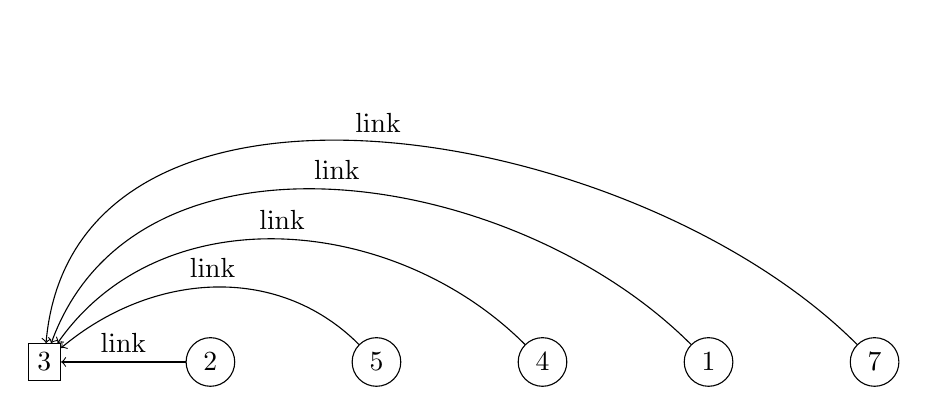
\begin{tikzpicture}[node distance=60pt]
\node [shape=rectangle, draw] (N3) {$3$};
\node [shape=circle, right of=N3, draw] (N2) {$2$};
\node [shape=circle, right of=N2, draw] (N5) {$5$};
\node [shape=circle, right of=N5, draw] (N4) {$4$};
\node [shape=circle, right of=N4, draw] (N1) {$1$};
\node [shape=circle, right of=N1, draw] (N7) {$7$};

\draw[->] (N2) -- (N3) node [midway, above] {link};
\draw[->] (N5) to [out=135, in=40] node [midway, above] {link} (N3);
\draw[->] (N4) to [out=135, in=55] node [midway, above] {link} (N3);
\draw[->] (N1) to [out=135, in=70] node [midway, above] {link} (N3);
\draw[->] (N7) to [out=135, in=85] node [midway, above] {link} (N3);
\end{tikzpicture}

\section*{Step 2 : $2$ outputs on $link$  to $3$}

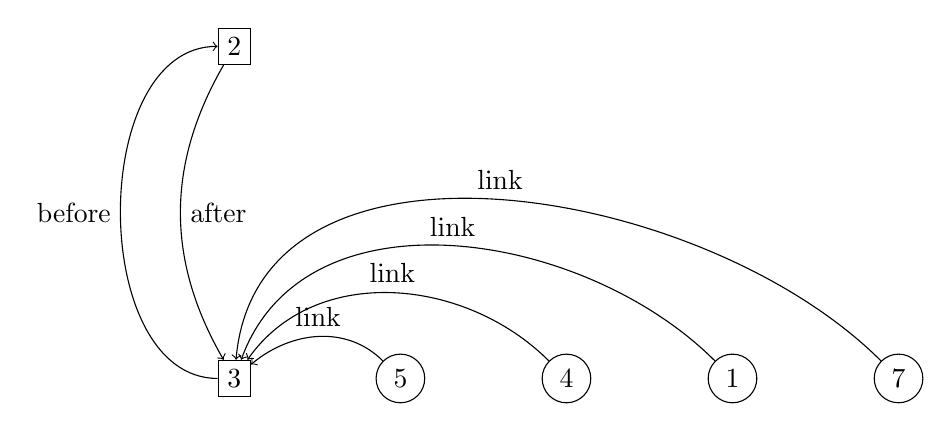
\begin{tikzpicture}[node distance=60pt]
\node [shape=rectangle, draw] (N2) {$2$};
\node [shape=rectangle, draw, below of=N2, node distance=120pt] (N3) {$3$};
\node [shape=circle, right of=N3, draw] (N5) {$5$};
\node [shape=circle, right of=N5, draw] (N4) {$4$};
\node [shape=circle, right of=N4, draw] (N1) {$1$};
\node [shape=circle, right of=N1, draw] (N7) {$7$};

\draw[->] (N2) to [out=-120, in=120] node [midway, right] {after} (N3);
\draw[->] (N3) to [out=180, in=-180] node [midway, left] {before} (N2);
\draw[->] (N5) to [out=135, in=40] node [midway, above] {link} (N3);
\draw[->] (N4) to [out=135, in=55] node [midway, above] {link} (N3);
\draw[->] (N1) to [out=135, in=70] node [midway, above] {link} (N3);
\draw[->] (N7) to [out=135, in=85] node [midway, above] {link} (N3);
\end{tikzpicture}

\section*{Step 3 : $1$ outputs on $link$  to $3$}

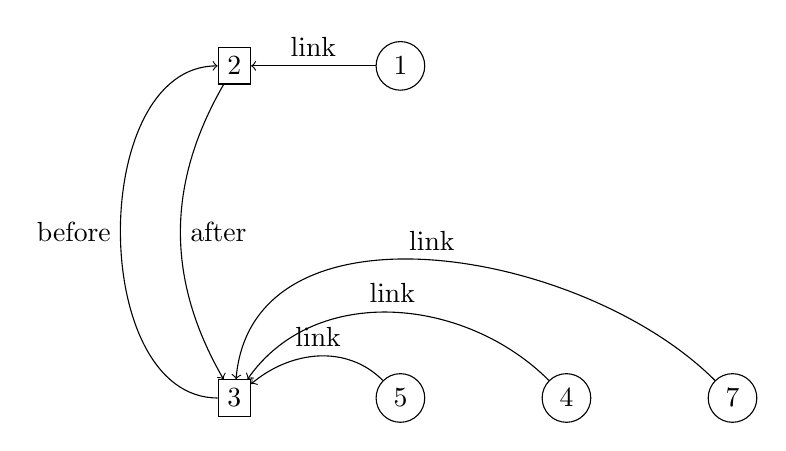
\begin{tikzpicture}[node distance=60pt]
\node [shape=rectangle, draw] (N2) {$2$};
\node [shape=rectangle, draw, below of=N2, node distance=120pt] (N3) {$3$};
\node [shape=circle, right of=N3, draw] (N5) {$5$};
\node [shape=circle, right of=N5, draw] (N4) {$4$};
\node [shape=circle, right of=N2, draw] (N1) {$1$};
\node [shape=circle, right of=N4, draw] (N7) {$7$};

\draw[->] (N2) to [out=-120, in=120] node [midway, right] {after} (N3);
\draw[->] (N3) to [out=180, in=-180] node [midway, left] {before} (N2);
\draw[->] (N5) to [out=135, in=40] node [midway, above] {link} (N3);
\draw[->] (N4) to [out=135, in=55] node [midway, above] {link} (N3);
\draw[->] (N1) to [out=180, in=0] node [midway, above] {link} (N2);
\draw[->] (N7) to [out=135, in=85] node [midway, above] {link} (N3);
\end{tikzpicture}

\section*{Step 4 : $4$ outputs on $link$  to $3$}

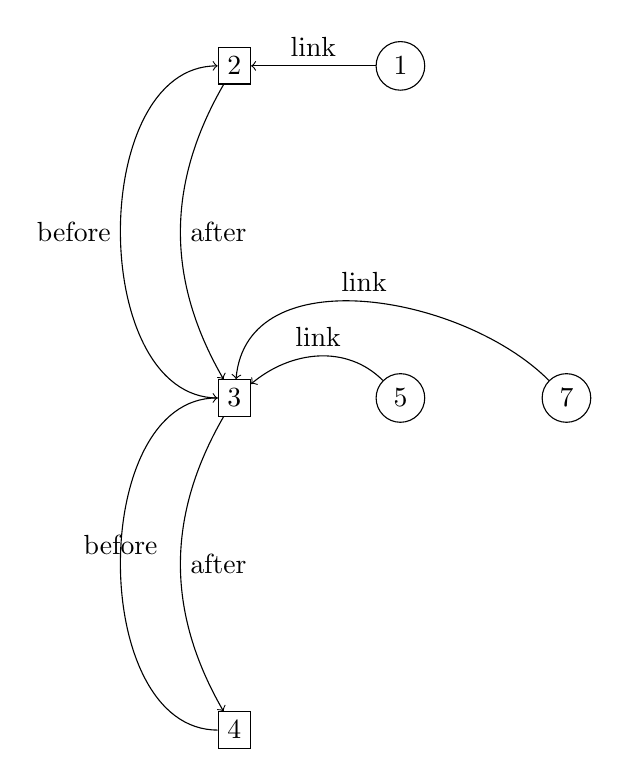
\begin{tikzpicture}[node distance=60pt]
\node [shape=rectangle, draw] (N2) {$2$};
\node [shape=rectangle, draw, below of=N2, node distance=120pt] (N3) {$3$};
\node [shape=rectangle, below of=N3, draw, node distance=120pt] (N4) {$4$};
\node [shape=circle, right of=N3, draw] (N5) {$5$};
\node [shape=circle, right of=N2, draw] (N1) {$1$};
\node [shape=circle, right of=N5, draw] (N7) {$7$};

\draw[->] (N4) to [out=180, in=-180] node [midway, above] {before} (N3);
\draw[->] (N3) to [out=-120, in=120] node [midway, right] {after} (N4);
\draw[->] (N2) to [out=-120, in=120] node [midway, right] {after} (N3);
\draw[->] (N3) to [out=180, in=-180] node [midway, left] {before} (N2);
\draw[->] (N5) to [out=135, in=40] node [midway, above] {link} (N3);
\draw[->] (N1) to [out=180, in=0] node [midway, above] {link} (N2);
\draw[->] (N7) to [out=135, in=85] node [midway, above] {link} (N3);
\end{tikzpicture}

\section*{Step 5 : $5$ outputs on $link$  to $3$}

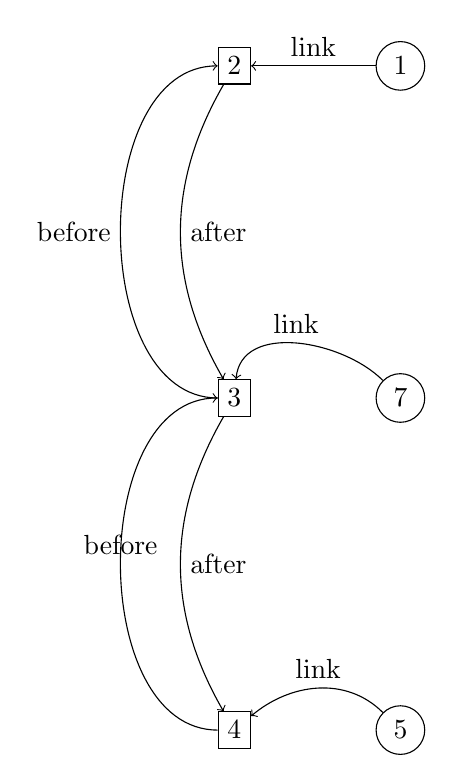
\begin{tikzpicture}[node distance=60pt]
\node [shape=rectangle, draw] (N2) {$2$};
\node [shape=rectangle, draw, below of=N2, node distance=120pt] (N3) {$3$};
\node [shape=rectangle, below of=N3, draw, node distance=120pt] (N4) {$4$};
\node [shape=circle, right of=N4, draw] (N5) {$5$};
\node [shape=circle, right of=N2, draw] (N1) {$1$};
\node [shape=circle, right of=N3, draw] (N7) {$7$};

\draw[->] (N4) to [out=180, in=-180] node [midway, above] {before} (N3);
\draw[->] (N3) to [out=-120, in=120] node [midway, right] {after} (N4);
\draw[->] (N2) to [out=-120, in=120] node [midway, right] {after} (N3);
\draw[->] (N3) to [out=180, in=-180] node [midway, left] {before} (N2);
\draw[->] (N5) to [out=135, in=40] node [midway, above] {link} (N4);
\draw[->] (N1) to [out=180, in=0] node [midway, above] {link} (N2);
\draw[->] (N7) to [out=135, in=85] node [midway, above] {link} (N3);
\end{tikzpicture}

\section*{Step 6 : $1$ outputs on $link$  to $2$}

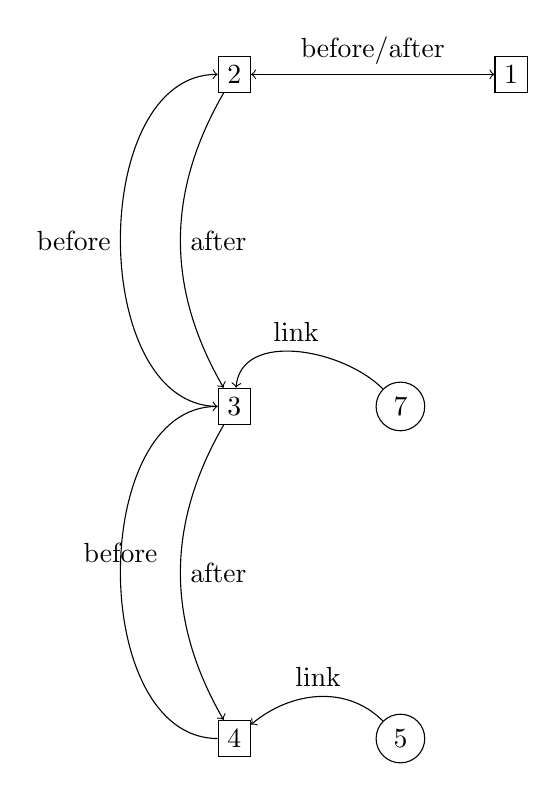
\begin{tikzpicture}[node distance=60pt]
\node [shape=rectangle, draw] (N2) {$2$};
\node [shape=rectangle, draw, below of=N2, node distance=120pt] (N3) {$3$};
\node [shape=rectangle, below of=N3, draw, node distance=120pt] (N4) {$4$};
\node [shape=circle, right of=N4, draw] (N5) {$5$};
\node [shape=rectangle, right of=N2, draw, node distance=100pt] (N1) {$1$};
\node [shape=circle, right of=N3, draw] (N7) {$7$};

\draw[->] (N4) to [out=180, in=-180] node [midway, above] {before} (N3);
\draw[->] (N3) to [out=-120, in=120] node [midway, right] {after} (N4);
\draw[->] (N2) to [out=-120, in=120] node [midway, right] {after} (N3);
\draw[->] (N3) to [out=180, in=-180] node [midway, left] {before} (N2);
\draw[->] (N5) to [out=135, in=40] node [midway, above] {link} (N4);
\draw[<->] (N1) to [out=180, in=0] node [midway, above] {before/after} (N2);
\draw[->] (N7) to [out=135, in=85] node [midway, above] {link} (N3);
\end{tikzpicture}

\section*{Step 7 : $7$ outputs on $link$  to $3$}

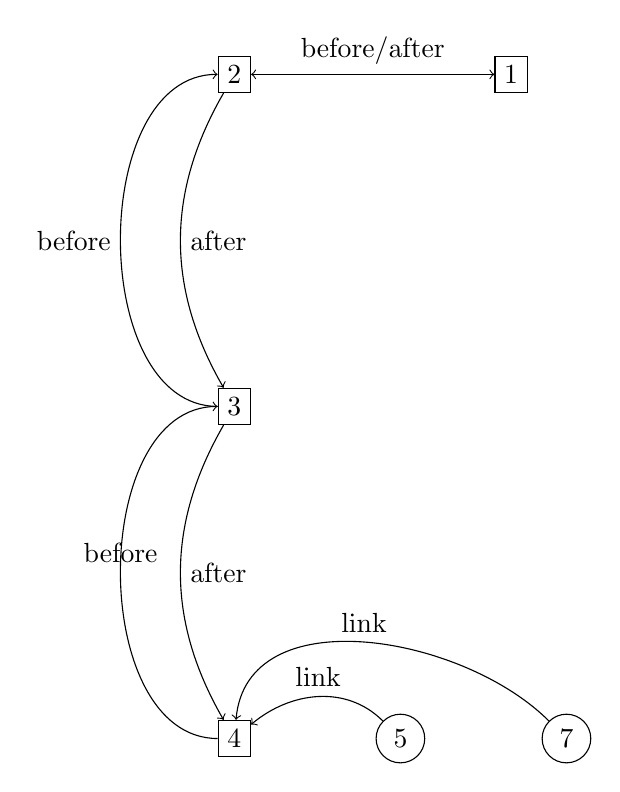
\begin{tikzpicture}[node distance=60pt]
\node [shape=rectangle, draw] (N2) {$2$};
\node [shape=rectangle, draw, below of=N2, node distance=120pt] (N3) {$3$};
\node [shape=rectangle, below of=N3, draw, node distance=120pt] (N4) {$4$};
\node [shape=circle, right of=N4, draw] (N5) {$5$};
\node [shape=rectangle, right of=N2, draw, node distance=100pt] (N1) {$1$};
\node [shape=circle, right of=N5, draw] (N7) {$7$};

\draw[->] (N4) to [out=180, in=-180] node [midway, above] {before} (N3);
\draw[->] (N3) to [out=-120, in=120] node [midway, right] {after} (N4);
\draw[->] (N2) to [out=-120, in=120] node [midway, right] {after} (N3);
\draw[->] (N3) to [out=180, in=-180] node [midway, left] {before} (N2);
\draw[->] (N5) to [out=135, in=40] node [midway, above] {link} (N4);
\draw[<->] (N1) to [out=180, in=0] node [midway, above] {before/after} (N2);
\draw[->] (N7) to [out=135, in=85] node [midway, above] {link} (N4);
\end{tikzpicture}

\section*{Etc ...}

\textbf{Remark} :  for termination, needs a $head$ process
 that is signaled each time a $link$ is destroyed, and the
 $before/after$ relation  (at least $after$) must also cover
 the $head$.


\end{document}